% ================================================================================
\documentclass{amsart}

%     If your article includes graphics, uncomment this command.
\usepackage{graphicx}
\usepackage{comment}
\usepackage{url}
\usepackage{hyperref}
\usepackage{float}

\usepackage{listings}
\lstset{
language=Python,
basicstyle=\small\sffamily,
%basicstyle=\tiny\sffamily,
numbers=left,
numberstyle=\tiny,
frame=tb,
%frame=single,
columns=fullflexible,
showstringspaces=false
}

\newtheorem{theorem}{Theorem}[section]
\newtheorem{lemma}[theorem]{Lemma}

\theoremstyle{definition}
\newtheorem{definition}[theorem]{Definition}
\newtheorem{example}[theorem]{Example}
\newtheorem{xca}[theorem]{Exercise}

\theoremstyle{remark}
\newtheorem{remark}[theorem]{Remark}

\numberwithin{equation}{section}

%    Absolute value notation
\newcommand{\abs}[1]{\lvert#1\rvert}

%    Blank box placeholder for figures (to avoid requiring any
%    particular graphics capabilities for printing this document).
\newcommand{\blankbox}[2]{%
  \parbox{\columnwidth}{\centering
%    Set fboxsep to 0 so that the actual size of the box will match the
%    given measurements more closely.
    \setlength{\fboxsep}{0pt}%
    \fbox{\raisebox{0pt}[#2]{\hspace{#1}}}%
  }%
}
% ================================================================================
% TODO: NOTES
\begin{comment}
    \lstinputlisting[basicstyle=\tiny]{files/snowflake_tree.txt}
\end{comment}
% ================================================================================
\begin{document}
% ================================================================================
\title{Snowflake audit\\ -\\ \small{Snapshot}}
% ================================================================================
\author{Carolin Z\"obelein}
\address{Carolin Z\"obelein, Independent mathematical scientist, Josephsplatz 8, 90403 N\"urnberg, Germany, \url{https://research.carolin-zoebelein.de}}
%\curraddr{}
\email{contact@carolin-zoebelein.de, PGP: D4A7 35E8 D47F 801F 2CF6 2BA7 927A FD3C DE47 E13B}
\thanks{The author believes in the importance of the independence of research and is funded by the public community. If you also believe in this values, you can find ways for supporting the author's work here: \url{https://research.carolin-zoebelein.de/crowdfunding.html}}
% ================================================================================
%\subjclass[2000]{Primary 54C40, 14E20; Secondary 46E25, 20C20}	% TODO
\date{Last change: \today, Status: Draft}
\dedicatory{This paper is dedicated to all the brave snowflakes who die every year during winter.}
%\keywords{Differential geometry, algebraic geometry}	% TODO
% ================================================================================
\begin{abstract} % TODO
	STATUS: DRAFT
\end{abstract}
% ================================================================================
\maketitle
% ================================================================================
\tableofcontents
% ================================================================================
\newpage
\section*{Preamble}
\label{s:preamble}
% --------------------------------------------------------------------------------
The following document is for discussion purposses only. It gives no warranty for completeness and correctness.
% ================================================================================
\section{Introduction}
\label{s:introduction}
% --------------------------------------------------------------------------------
\textit{Snowflake} is a pluggable transport, which uses WebRTC to proxy traffic through emporary proxies. It aims to work kind of like flash proxy \cite{SnowflakeEmail} \cite{SnowflakeGitWeb}. This document is a short snapshot audit of the current state of the existing snowflake code  \cite{SnowflakeGit} on \url{https://gitweb.torproject.org/pluggable-transports/snowflake.git/}.
% ================================================================================
\section{Basic package structure}
\label{s:basicpackagestructure}
% --------------------------------------------------------------------------------
At first, let's have a first look at the basic package structure of Snowflake \cite{SnowflakeGit}.
% --------------------------------------------------------------------------------
\subsection{General package information}
\label{ss:generalpackageinformation}
% --------------------------------------------------------------------------------
\textit{Snowflake} is a \textit{Go}-based Pluggable Transport using WebRTC, inspired by Flashproxy.
% --------------------------------------------------------------------------------
\subsection{Package tree}
\label{ss:packagetree}
% --------------------------------------------------------------------------------
Given are the following main parts of the package:
\begin{itemize}
    \item \textbf{appengine (d)}: Runs an Google App Engine and reflects domain-fronted requests from a client to the Snowflake broker.
    \item \textbf{broker (d)}: Handles the rendezvous by matching Snowflake clients with proxies. It passes the client's WebRTC session descriptions. So the clients and proxies can establish a peer connection.
    \item \textbf{client (d)}: Tor client component of Snowflake.
    \item \textbf{proxy (d)}: Browser proxy component of Snowflake.
    \item \textbf{proxy-go (d)}: Standalone version of the Snowflake proxy.
    \item \textbf{server (d)}: Server transport plugin for Snowflake. The client connects to the proxy using WebRTC and the proxy connects to the server using WebSocket.
    \item \textbf{server-webrtc (d)}: WebRTC server plugin which uses an HTTP server that simulates the interaction that a client would have with the broker, for direct testing.
    \item \textbf{CONTRIBUTING.md (f), LICENSE (f), README.md (f):} Standard package files.
\end{itemize}

d= directory, f=file.
% --------------------------------------------------------------------------------
\subsection{Interaction structure}
\label{ss:interactionstructure}
% --------------------------------------------------------------------------------
In figure \ref{fig:interactionstructure} you can see the interaction structure between the different parts of Snowflake.

\begin{figure}[H]
\centering
    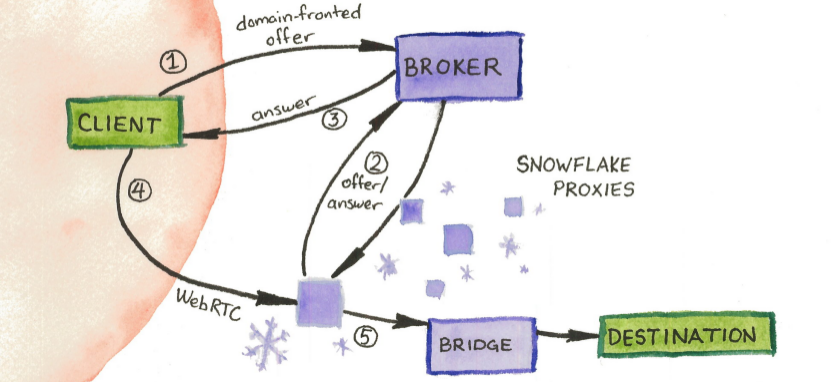
\includegraphics[width=0.8\textwidth]{images/snowflake-schematic.png}
\caption{Schematic graphic of the interaction structure of Snowflake. Taken from \cite{SnowflakeSchematic}.}
\label{fig:interactionstructure}
\end{figure}

\begin{itemize}
    \item [1a.] The client makes a request to the broker.
    \item [1b.] The appengine reflects the domain-fronted request from the client to the broker.
    \item [2a.] The broker matches the client with proxies.
    \item [2b.] The broker passes the client's WebRTC session descriptions.
    \item [3.] The broker gives an answer about the matching proxy to the client.
    \item [4.] The client uses WebRTC for the connection to the given proxy.
    \item [5.] Finally, the client connects to a bridge over WebRTC.
\end{itemize}
% ================================================================================
\section{Client}
\label{s:client}
% --------------------------------------------------------------------------------
In the following sections we will do a raw audit of the Snowflake client.
% --------------------------------------------------------------------------------
\subsection{README and torrc files}
\label{ss:readmeandtorrcfiles}
% --------------------------------------------------------------------------------
Given are the \textit{README.md}, \textit{torrc}, \textit{torrc-localhost} and \textit{torrc-manual} files which contain similar content.

\begin{figure}[H]
\begin{lstlisting}[frame=single, language=C, caption=torrc-Config: Standard values]
UseBridges 1
DataDirectory datadir

Bridge snowflake 0.0.3.0:1
\end{lstlisting}
\label{fig:torrcconfigstandardvalues}
\end{figure}

In listing \ref{fig:torrcconfigstandardvalues} are defined the three standard values \cite{TorStableManual}.
\begin{itemize}
    \item \textbf{UseBridges 1}: Tor will fetch descriptors for bridges.
    \item \textbf{DataDirectory datadir}: Store working data in datadir. Can not be changed while tor is running.
    \item \textbf{Bridge snowflake 0.0.3.0:1}: When set along with UseBridges, instructs Tor to use the relay at "IP:ORPort" as a "bridge" relaying into the Tor network. If "transport" is provided, it must match a ClientTransportPlugin line. We then use that pluggable transport’s proxy to transfer data to the bridge, rather than connecting to the bridge directly.
\end{itemize}

The Snowflake client torrc default values are

\begin{figure}[H]
\begin{lstlisting}[frame=single, language=C, caption=torrc-Config: Snowflake client default values]
ClientTransportPlugin snowflake exec ./client \
-url https://snowflake-broker.azureedge.net/ \
-front ajax.aspnetcdn.com \
-ice stun:stun.l.google.com:19302
\end{lstlisting}
\label{fig:torrcconfigsnowflakeclientdefault}
\end{figure}

and can also be found in the client-\textit{README.md} \cite{SnowflakeGitClient}

\begin{itemize}
    \item \textbf{-url}: Should be the URL of a Broker instance. This is required to have
automated signalling (which is desired in most use cases).
When omitted, the client uses copy-paste signalling instead.
    \item \textbf{-front}: An optional front domain for the Broker request.
    \item \textbf{-ice }: A comma-separated list of ICE servers. These can be STUN or TURN
servers.
\end{itemize}

. Additionally the following values can be set (see also \textit{snowflake.go} \cite{SnowflakeGitClient}).

\begin{figure}[H]
\begin{lstlisting}[frame=single, language=C, caption=torrc-Config: Snowflake client additional values]
-max 3
-log snowflake.log
\end{lstlisting}
\label{fig:torrcconfigsnowflakeclientadditional}
\end{figure}

\begin{itemize}
    \item \textbf{-max}: Capacity for number of multiplexed WebRTC peers.
    \item \textbf{-log}: Name of log file.
\end{itemize}
% ================================================================================
\section{Broker}
\label{s:broker}
% --------------------------------------------------------------------------------
In the following sections we will do a raw audit of the Snowflake broker.
% ================================================================================
\section{Appengine}
\label{s:appengine}
% --------------------------------------------------------------------------------
In the following sections we will do a raw audit of the Snowflake appengine.
% ================================================================================
\section{Proxy-go}
\label{s:proxygo}
% --------------------------------------------------------------------------------
In the following sections we will do a raw audit of Snowflake's proxy-go.
% ================================================================================
\section{Conclusion}
\label{s:conclusion}
% --------------------------------------------------------------------------------
% TODO
% ================================================================================
% Bibliography
\nocite{*}
%\bibliographystyle{amsplain}
\bibliographystyle{unsrtdin}
\bibliography{snowflake-audit}
% ================================================================================
\section*{License}
\label{s:license}
% --------------------------------------------------------------------------------
\begin{center}
	
\includegraphics{by-nc-nd.png} \\
	\url{https://creativecommons.org/licenses/by-nc-nd/4.0/}
\end{center}
% ================================================================================
\end{document}
% ================================================================================
